\documentclass{article}
\usepackage{amsmath}
\usepackage{graphicx}
\usepackage{subfig}


\begin{document}
\title{PP3 Report}
\author{Logan Bontrager}
\maketitle

\section*{Task 1)}

In the first task, we implement a generative and bayesian logistic regression model on various datasets. For each dataset, we train the model 30 times stochastically on various training sizes of data. We then compute the mean error and standard deviation of this error for each method at each size and on each dataset. The results are given in the graphs below where the generative model is represented by the left column and the bayesian the right.
\\
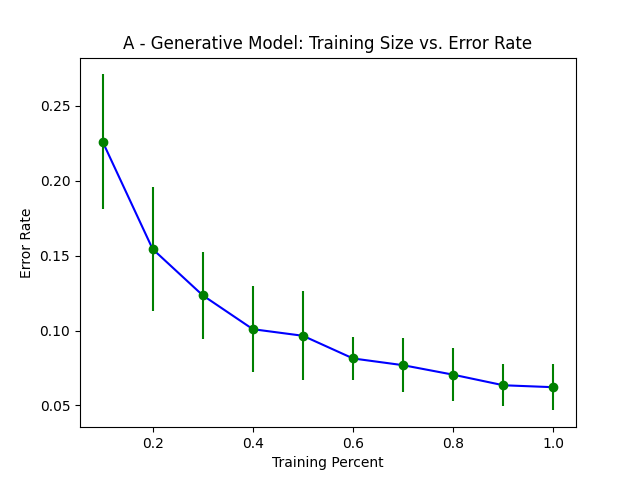
\includegraphics[width=0.5\textwidth]{../output/generative-A.png}
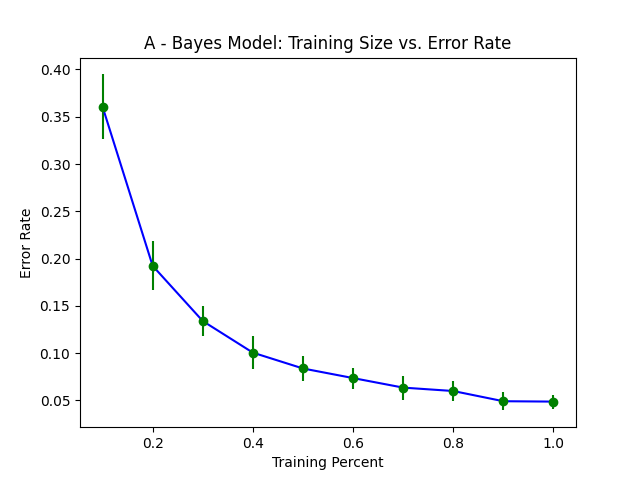
\includegraphics[width=0.5\textwidth]{../output/bayes-A.png}
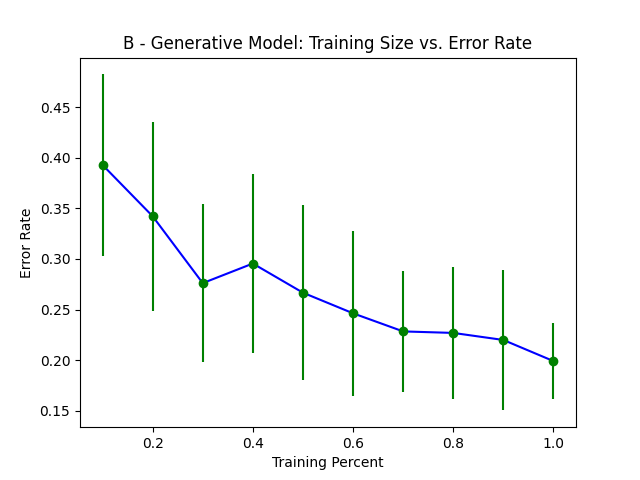
\includegraphics[width=0.5\textwidth]{../output/generative-B.png}
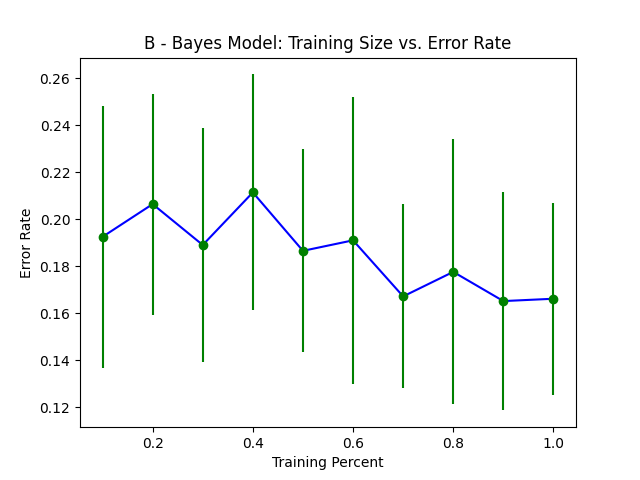
\includegraphics[width=0.5\textwidth]{../output/bayes-B.png}
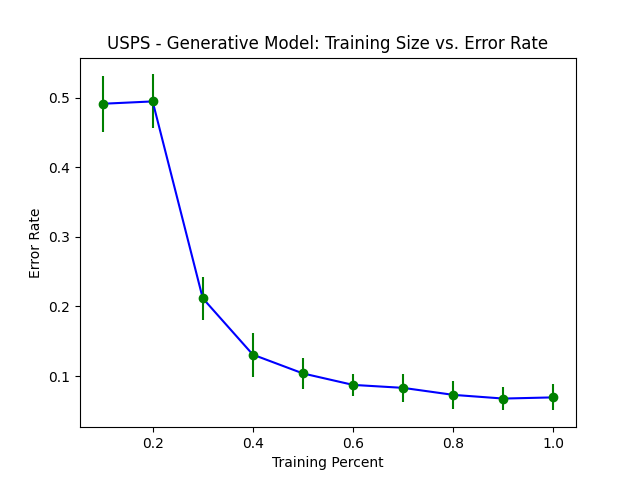
\includegraphics[width=0.5\textwidth]{../output/generative-USPS.png}
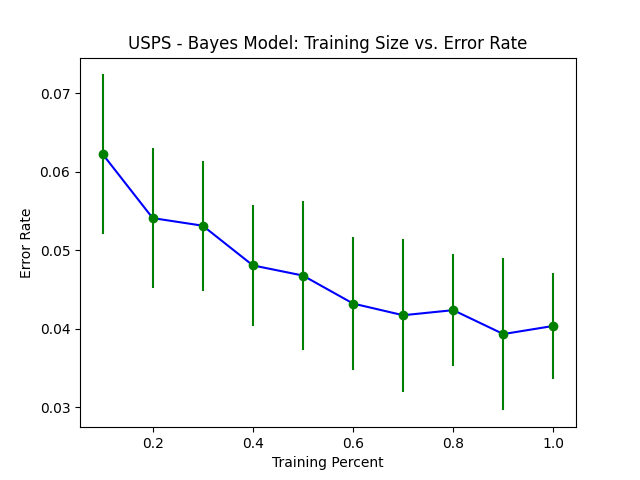
\includegraphics[width=0.5\textwidth]{../output/bayes-USPS.png}
\\ \\
Upon analyzing the data, it appears that the bayesian model's test error converges quicker and potentially more steadily as a function of training size. This is likely due to the prior taken over the data which could help normalize the results under the random sampling and little training data. In terms of holistic performance, the algorithms perform quite similarly and appear to have a near identical error rate when using larger training sizes. On smaller training proportions, we see more variation in results between the two. One thing to note is that the performance of the models don't seem to decrease as much relative to the increasing training size on the B dataset when compared to others.

\section*{Task 2)}

In the second task, we evaluate the convergence qualities of both newton's method and gradient ascent under the bayesian logistic regression model. This translates to analyzing the rate at which the weight vector converges in terms of time and the final weight vector itself. The results are given in the graph below.

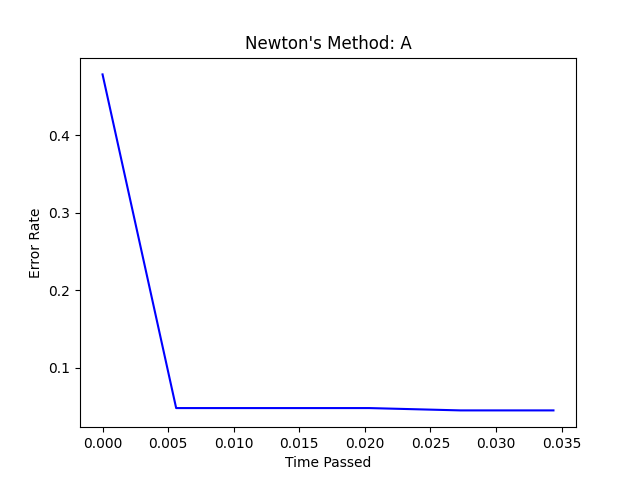
\includegraphics[width=0.5\textwidth]{../output/newton-A.png}
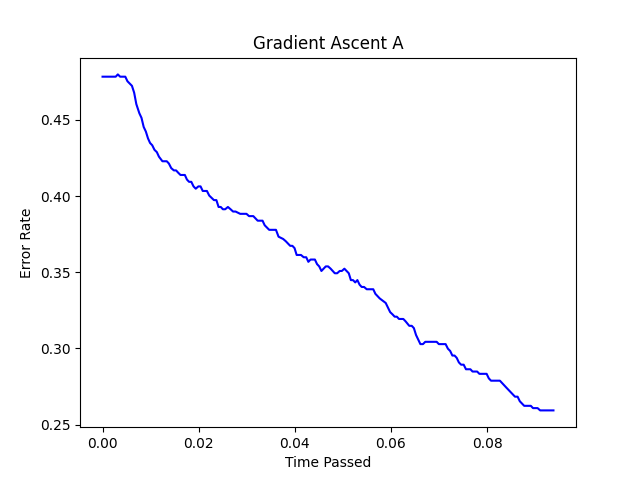
\includegraphics[width=0.5\textwidth]{../output/gradient-A.png}
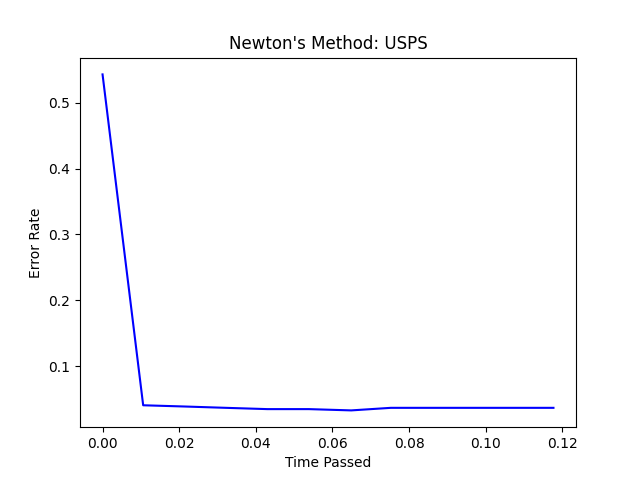
\includegraphics[width=0.5\textwidth]{../output/newton-USPS.png}
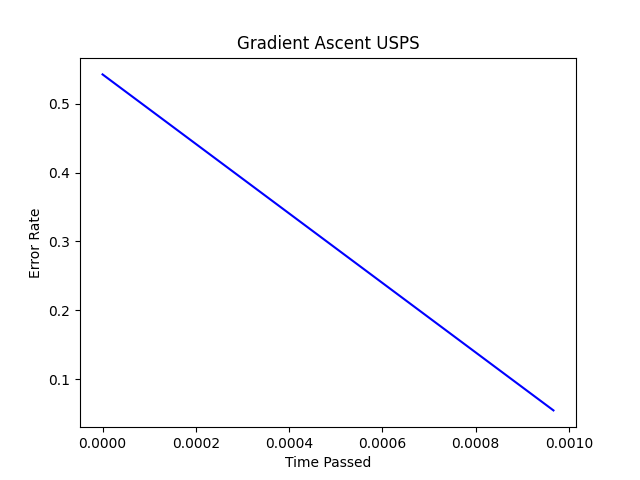
\includegraphics[width=0.5\textwidth]{../output/gradient-USPS.png}
\\ \\
From the graph, we can see that the newton's method converges much quicker relative to time than gradient ascent. In terms of gradient ascent on the USPS dataset, the algorithm converges almost instantaniously compared to dataset A. I believe that this is due to the characterisitics of the data and is the reason we see a straignt line, i.e., the algo satisfies the stopping criteria within 10 iterations. When considering performance, both methods acheive near identical test errors on USPS but not on dataset A. If given more stringent stopping criteria, I believe performance would be similar on A.


\end{document}